Our evaluation illustrates key findings about \sys. We show that: \todo{Make a list of core findings here once results are solid}{Przemek}

\subsection{\sys Runtime Performance}
\label{sec:results_evaluation}

Our aim is to assess \sys as detailed as possible. For this we have characterized \sys runtime performance (execution time), based on a set of benchmarks, considering core task adaptation mechanisms of \sys: \emph{task coalescing} and \emph{task downscaling}. We also characterize \sys overhead showing precisely what is the source of \sys superior performance. Additionally, we characterize \sys code. 

\sys is compared to Alpaca runtime. We remind the reader that the benchmarks for Alpaca were hand-transformed in a time-consuming manual process from Clang (LLVM-generated code) to GCC (see Section~\ref{sec:implementation}). The manual code transformation was required as \sys was written with GCC in mind, and Alpaca cannot support any other complier than LLVM.

\subsubsection{\sys Task Adaptation}
\label{sec:result_coalescing}

We characterize \sys by studying how its performance varies due to task adaptation. We start with evaluating the task coalescing mechanism.

\textbf{Coalescing Strategies Performance.} We first need to assess the performance of all coalescing strategies introduced in Section~\ref{sec:task_coalescing}. Figure~\ref{fig:coalescing} shows the run time of \sys's three coalescing strategies normalized to the \sys runtime without coalescing. \todo{Check if this normalization is true}{Przemek} We show data from experiments measured at 15\,cm WISP to RF generator antenna distance. The results show the benefit from coalescing for all applications. The difference in performance between all strategies is highly application-dependent. The gain from energy and task-aware strategy (EA, smart) compared to task-aware only (TA, fast) are particularly small (or negative) for applications with large task sizes, i.e. \textbf{fft}. \todo{Provide more justification}{Przemek}

%\begin{wrapfigure}{t!}{0.5\textwidth}
\begin{figure}
	\centering
	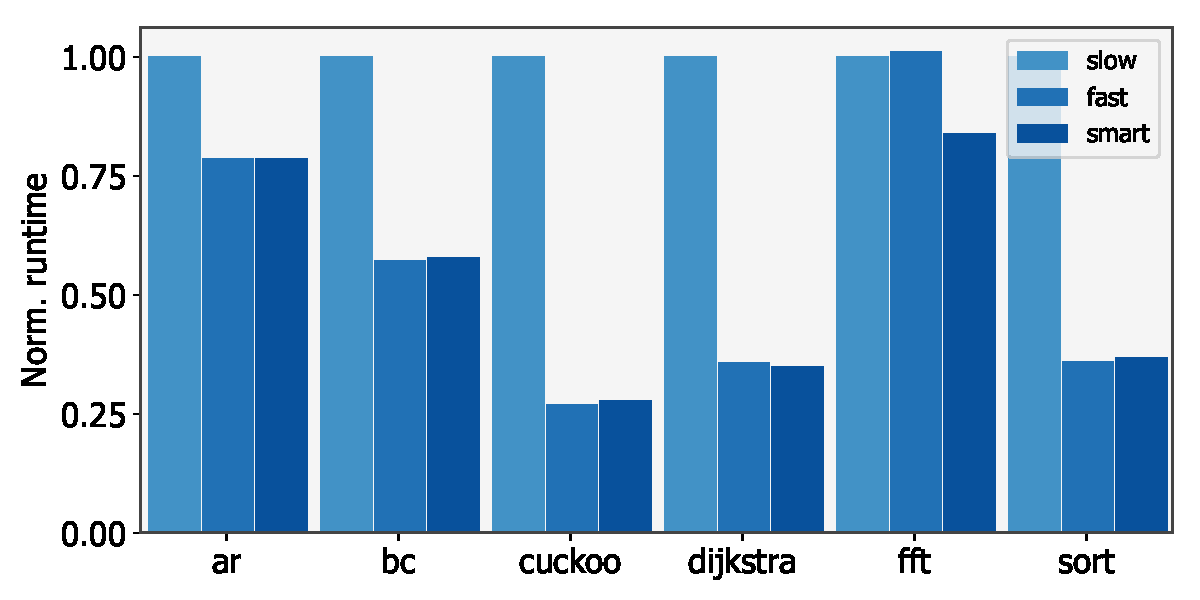
\includegraphics[width=\columnwidth]{figures/coalStrategies}
	\caption{\sys coalescing strategies performance per application on intermittent power (RF generator at 15\,cm from the WISP) compared to \sys without coalescing. \sys task coalescing strategy provides significant improvements (from 0.25, \textbf{ar}, up to 0.70, \textbf{sort}) compared to a non-coalesced system. \todo{no coalescing missing; change names of algos; reduce Y width by 40\%; names of apps bold}{Przemek}}
	\label{fig:coalescing}
\end{figure}
%\end{wrapfigure}

\textbf{\sys versus Task-based Model.} We now evaluate \sys's run time performance and compare \sys to the run time performance of Alpaca. Results are given in Figure~\ref{fig:runtime}. For each application we measured its execution time using real wireless power provisioned from the RF signal generator at three distances (refer again to Section~\ref{sec:implementation}).

The data show the average execution time of each application with runtimes normalized to \sys's average. The results show that \sys provides a performance benefit compared to Alpaca for most applications (all except for \textbf{ar} and \textbf{cuckoo}). The performance benefit is greatest for applications that have small tasks (\textbf{bc}, \textbf{sort}, \textbf{dijkstra}) at all distances on intermittent power. In applications that have larger tasks or access more different memory pages, \sys incurs overhead from memory virtualization that cause its performance to be comparable to (or worse than) Alpaca.

\begin{figure}
	\centering
	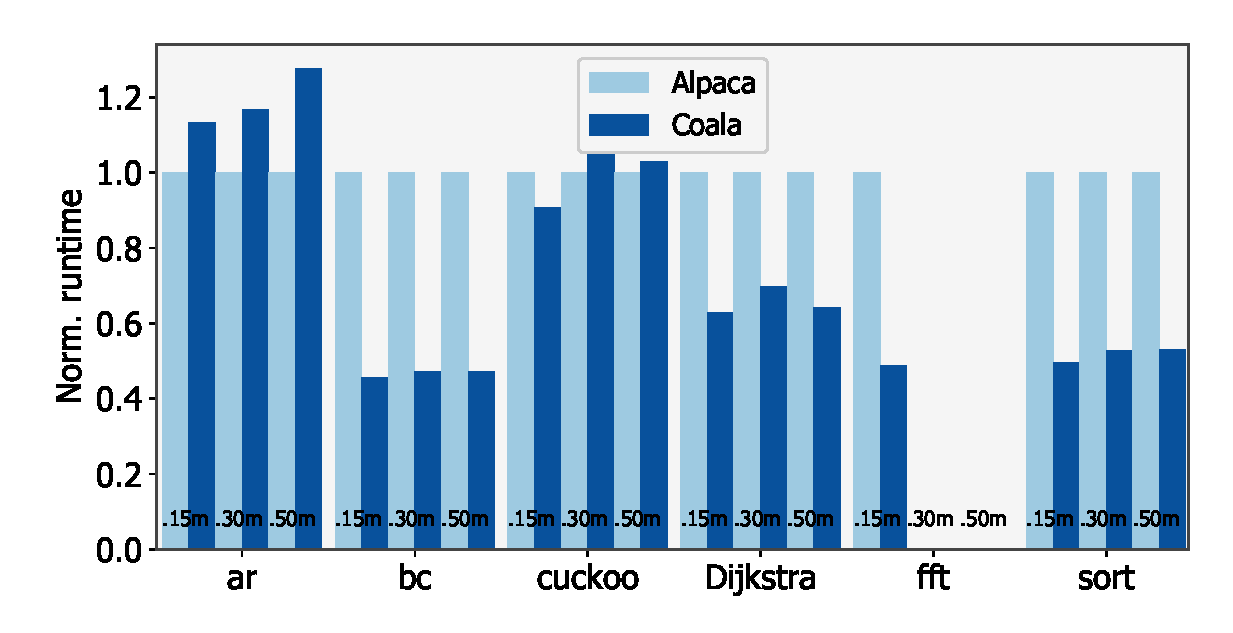
\includegraphics[width=\columnwidth]{figures/coala_alpaca_gcc}
	\caption{Performance of \sys applications at multiple WISP to RF generator antenna distances ()\{0.15, 0.3, 0.5\}\,m (left, center and right-most bar per application, respectively), compared against Alpaca (results normalized).}
	\label{fig:runtime}
\end{figure}

The data also illustrate that coalescing improves \sys's performance by eliminating the overhead of committing after each task. The performance benefit varies, providing up to 4.5x performance improvement. The cuckoo application (like other top-performers, bc and sort) has small tasks that \sys can easily coalesce to eliminate many commits. In contrast, for some applications, e.g. cem, coalescing does not improve performance. The reason for cem's poor performance is that cem uses a large LZW dictionary structure that spans multiple pages, but has very little {\em locality}. The absence of locality means that coalesced tasks do not access the same pages, and as a result, do not amortize commit overhead. The lack of locality causes performance to regress to be similar to the non-coalescing case. 

\textbf{Task Downscaling.} \todo{Provide text; add results}{Przemek}

\subsubsection{Characterization of \sys Overhead}
\label{sec:coala_overhead}

%Then, we need to know how many tasks \sys can coalesce within a given execution scenario. We ran a subset of applications (split by tasks manually) with continuous power supply and measured the size of tasks for each application and the amount of tasks coalesced. Result is given in Table~\ref{tab:aveVirtuTaskSize}. We see clearly that \sys manages to coalesce more tasks as individual tasks are small. As the size of individual task increases, e.g., as in the case of dft application, the number of coalesced tasks is also small. This result clearly shows that for the benefit of coalescing and for code portability, initial code should be split by \emph{as small tasks as possible}. This will help \sys to find the best possible virtual task size to minimise its runtime.

\indent \textbf{Overall \sys Overhead Breakdown.} The result is presented in Figure~\ref{fig:overallOverheadBreakdown}.

\begin{figure}
	\centering
	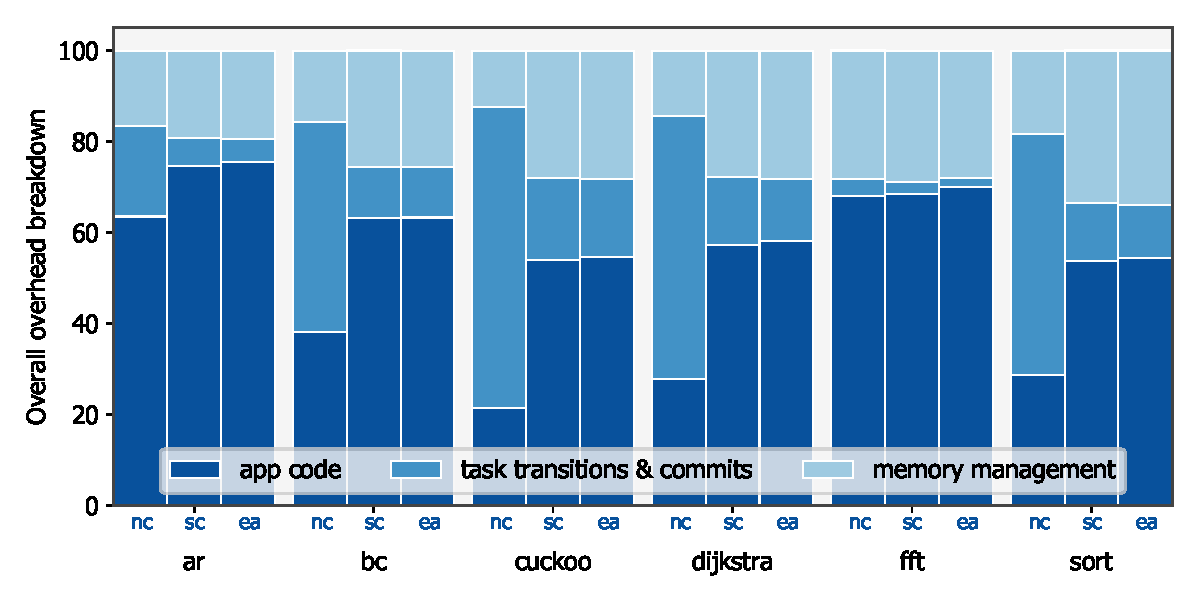
\includegraphics[width=\columnwidth]{figures/overallOverhead}
	\caption{Overall \sys overhead breakdown; nc: no coalescing, sc: slow coalescing, ea: energy-aware coalescing.}
	\label{fig:overallOverheadBreakdown}
\end{figure}

\textbf{\sys Coalescing Algorithm Efficiency.} The result is presented in Figure~\ref{fig:coalEfficiency}.

\begin{figure}
	\centering
	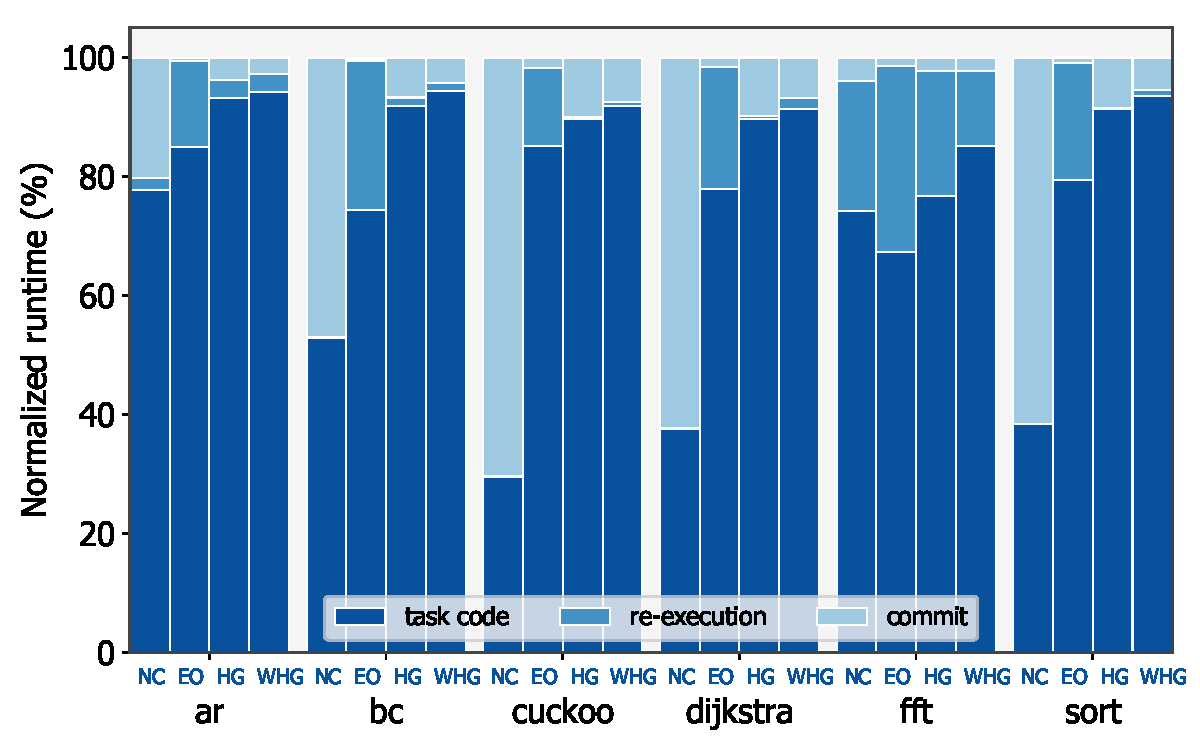
\includegraphics[width=\columnwidth]{figures/coalEfficiency}
	\caption{\sys coalescing algorithm efficiency; nc: no coalescing, sc: slow coalescing, ea: energy-aware coalescing, eta: energy and task-aware coalescing.}
	\label{fig:coalEfficiency}
\end{figure}

\textbf{\sys Memory Access Overhead Breakdown.} The result is presented in Figure~\ref{fig:coalmemory}.

\begin{figure}
	\centering
	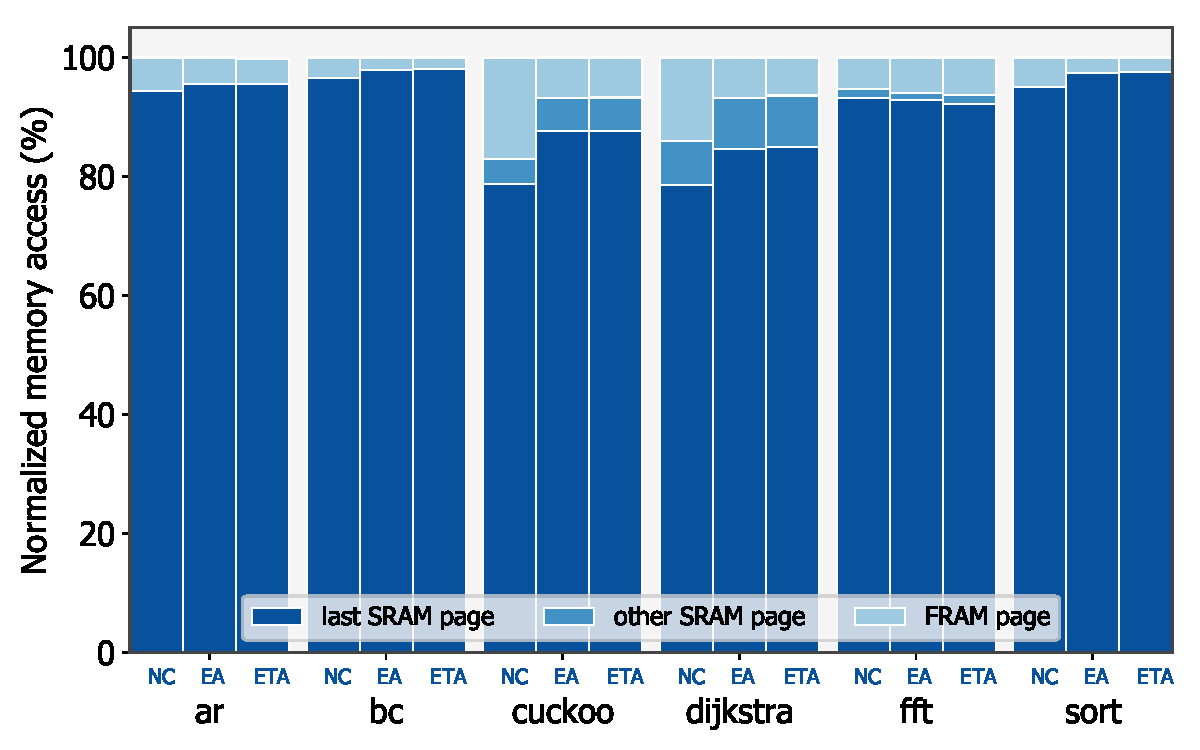
\includegraphics[width=\columnwidth]{figures/memAccess}
	\caption{\sys memory access overhead breakdown; nc: no coalescing, sc: slow coalescing, ea: energy-aware coalescing.}
	\label{fig:coalmemory}
\end{figure}

\subsubsection{\sys Paging Performance}
\label{sec:results_memory_management}

We evaluated the effect that paging with different page sizes has on \sys's performance and we show data in Figure~\ref{fig:page_size}; The top plot shows the run time performance normalized to the best per-application performance, using pages of different sizes in \sys, indicated with the labels at each bar; the bottom plot shows the number of page faults for the same set of executions normalized to the maximum of each set. We measured performance as MCU clock cycles using values read out by TI's CCS IDE. The results show a clear ``bathtub curve'' in the performance of each application, as the number of page faults varies. The data show that across application there is a page size that minimizes \emph{both} execution time. We observe that the page size is not the same for each application, although 64 byte pages perform well for all applications. The increased rate of page faults is responsible for the overhead with small page sizes; smaller pages require accessing more different pages, leading to higher paging costs. With larger page sizes, the overhead is higher than with moderate pages, too. The explanation for these higher overheads is that large pages have a higher commit cost. Even if an application accesses few memory locations, \sys pages data at full page size, degrading performance by sometimes paging in and out unnecessary data. The data reveal a reasonable default page size of 64 bytes and when developing an application, a developer should consider varying the page size to moderate poor performance.

\begin{figure}
	\centering
	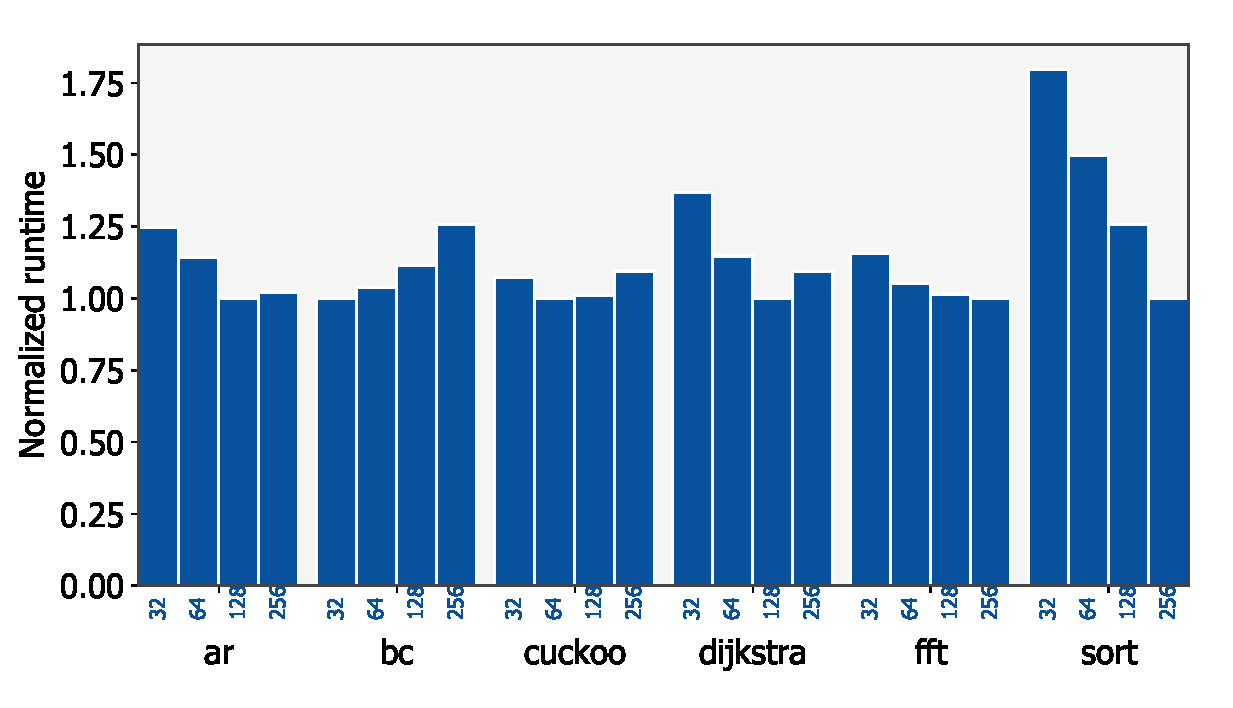
\includegraphics[width=\columnwidth]{figures/page_exec-time}
	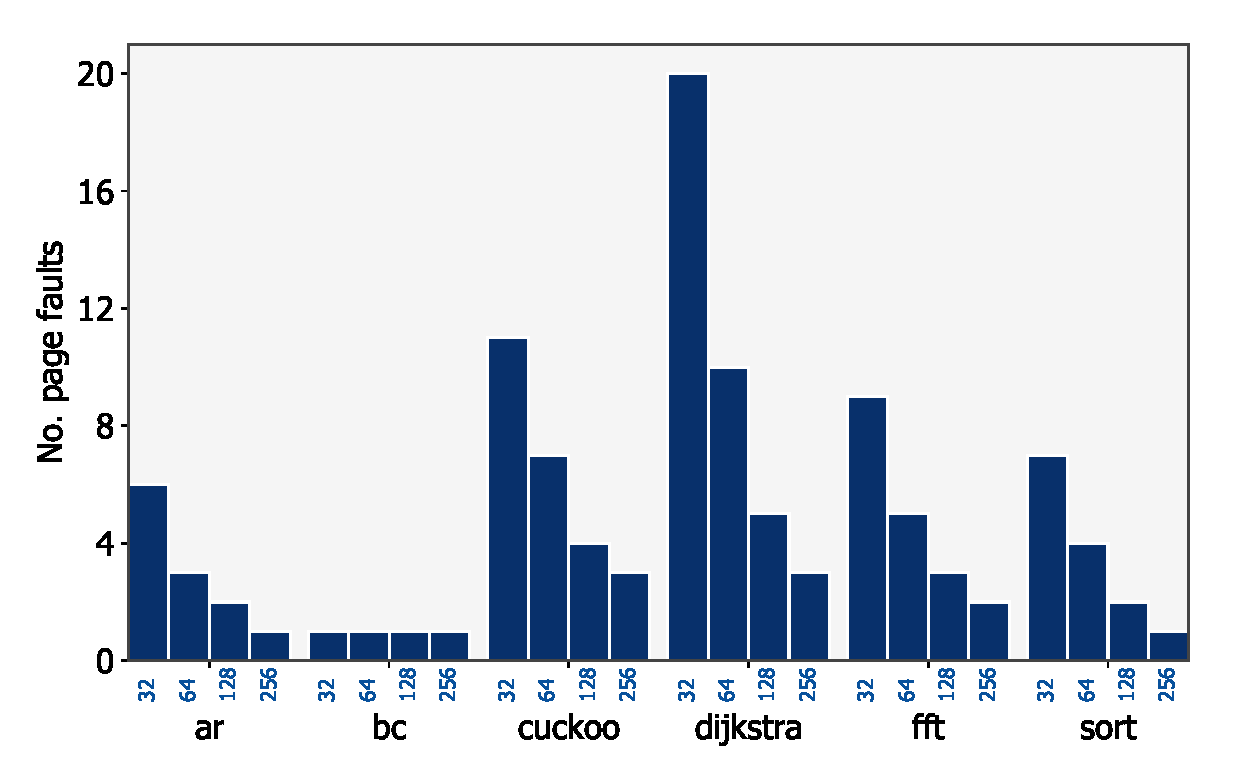
\includegraphics[width=\columnwidth]{figures/pagePulls}
	\caption{\textbf{\sys normalized runtime for various page sizes, \{32, 64,128,256\}\,bytes, per application (top) and respective page pulls (bottom)}).}\vspace{-0.5cm}
%\todo{change X to 0, remove the definition of X from caption}{Amjad}}
	\label{fig:page_size}
\end{figure}

%\subsection{\sys Memory Footprint?}
%\label{sec:results_program_characterization}
%
%\sys program characterization is provide in Table~\ref{table:compiler_result}. \todo{Finalize this section}{Przemek}
%
%\begin{table}
%	\begin{tabular}{| c | c | c | c | c |}
%		\hline
%		\multirow{2}{*}{Application} & \multicolumn{2}{ c |}{Memory footprint} & \multirow{2}{*}{No. tasks} & \multirow{2}{*}{SLOC} \\
%		\cline{2-3}
%		{} & \sys & Alpaca & {} & {} \\
%		\hline\hline
%				\textbf{ar} & --- & --- & --- & ---\\
%		\hline
%				\textbf{bc} & --- & --- & --- & ---\\
%		\hline
%				\textbf{cuckoo} & --- & --- & --- & ---\\
%		\hline
%				\textbf{dijkstra} & --- & --- & --- & ---\\
%		\hline
%				\textbf{fft} & --- & --- & --- & ---\\
%		\hline
%				\textbf{sort} & --- & --- & --- & ---\\
%		\hline
%	\end{tabular}
%		\caption{Comparison between \sys and Alpaca benchmarks.}
%		\label{table:compiler_result}\vspace{-0.5cm}
%\end{table}

%\begin{table}[t]
%	\centering
%	\renewcommand{\tabcolsep}{1pt}
%	\begin{tabular}{|l|cc|cc|cc|cc|c|}
%		\hline
%		{} & \multicolumn{2}{c|}{{\bf Prot. bytes}} & \multicolumn{2}{c|}{{\bf \# Tasks}} & \multicolumn{2}{c|}{{\bf \# Prot. acc.}} & \multicolumn{2}{c|}{\bf SLOC} & {\bf Comp.} \\
%		App & Man. & Comp. & Man. & Comp. & Man. & Comp. & \multicolumn{1}{l}{\sys} & \multicolumn{1}{r|}{Chain~\cite{chain}} & {\bf time} \\
%		\hline\hline
%		bc & 22 & 22 & 10 & 15 & 81 & 93 & 351 &588 & 3\\
%		cem & 3492 & 3242 & 12 & 9 & 92 & 123 & 388 &721 & 2\\
%		cuckoo & 282 & 288 & 15 & 6 & 90 & 76 & 483 &762 & 6\\
%		rsa & 332 & 250 & 20 & 27 & 130 & 296 & 887 &1233 & 86\\
%		ar & 166 & 218 & 11 & 6 & 112 & 333 & 483 &762 & 34\\
%		sort & 104 & 104 & 4 & 2 & 70 & 23 & 180 & 287 & $<$1\\
%		dft$^\dagger$ & --- & --- & --- & --- & --- & --- & 222 & 293 & ---\\
%		%dd &  &  &  &  &  &  &  & 287 &  \\
%		\hline
%	\end{tabular}
%		\caption{Comparison between \sys and Alpaca benchmarks.}
%		\label{table:compiler_result}\vspace{-0.5cm}
%\end{table}
